
    
    
    
    

%~\par
%\newpage 

    

    
    (some) LaTeX environments for Jupyter notebook
% No prompt!
%\textbf{Input \#{}}%
\begin{lstlisting}
%%javascript 
IPython.utils.load_extensions('calico-document-tools');
\end{lstlisting}% No prompt!
%\textbf{Output \#{}}
%
    
    \begin{verbatim}
<IPython.core.display.Javascript object>
\end{verbatim}

    % No prompt!
%\textbf{Input \#{}}%
\begin{lstlisting}
%%html
<style>
    .prompt{
        display: none;
</style>
\end{lstlisting}
    \section{Presentation and main
features}\label{presentation-and-main-features}

    This extension for IPython 3.x or Jupyter enables to use some LaTeX
commands and environments in the notebook's markdown cells.

\begin{enumerate}
\item \textbf{LaTeX commands and environments}

\begin{itemize}
\item support for some LaTeX commands within markdown cells, \emph{e.g.}
\texttt{\textbackslash{}textit}, \texttt{\textbackslash{}textbf},
\texttt{\textbackslash{}underline} \item support for
\textbf{theorems-like environments} \item support for \textbf{lists}:
\emph{enumerate, itemize},\\\item limited support for a \textbf{figure
environment}, \item support for an environment \emph{listing}, \item
additional \emph{textboxa} environment
\end{itemize}

\item \textbf{Citations and bibliography}

\begin{itemize}
\item support for \texttt{\textbackslash{}cite} with creation of a
References section
\end{itemize}

\item \textbf{Document-wide numbering of equations, support for
\texttt{\textbackslash{}label} and \texttt{\textbackslash{}ref}} \item
\textbf{Configuration toolbar} \item Styles can be customized in the
\emph{latex\_env.css} stylesheet
\end{enumerate}

A simple illustration is as follows: on can type the following in a
markdown cell

\begin{listing}
\begin{theorem} \label{theo:dotp}
Let $u$ and $v$ be two vectors of $\mathbb{R}^n$. The dot product can be expressed as
\begin{equation}
\label{eq:dotp}
u^Tv = |u||v| \cos \theta,
\end{equation}
where $\theta$ is the angle between $u$ and $v$ ...
\end{theorem}
\end{listing}

and have it rendered as

\begin{theorem}
\label{theo:dotp} Let $u$ and $v$ be two vectors of
$\mathbb{R}^n$. The dot product can be expressed as

\begin{equation}
\label{eq:dotp}
u^Tv = |u||v| \cos \theta,
\end{equation}

where $\theta$ is the angle between $u$ and $v$ \ldots{}
\end{theorem}

    \subsection{Implementation principle}\label{implementation-principle}

    The main idea is to override the standard Markdown renderer in order to
add a \emph{small} parsing of LaTeX expressions and environments. This
heavily uses regular expressions. The LaTeX expression are then rendered
using an html version. For instance
\texttt{\textbackslash{}underline\ \{something\}} is rendered as
\texttt{\textless{}u\textgreater{}\ something\ \textless{}/u\textgreater{}},
that is \underline{something}. The environments are replaced by an html
tag with a class derived from the name of the environment. For example,
a \texttt{definition} denvronment will be replaced by an html rendering
corresponding to the class \texttt{latex\_definition}. The styles
associated with the different classes are sepcified in
\texttt{latex\_env.css}. These substitutions are implemented in
\texttt{thsInNb4.js}.

    \subsection{Support for simple LaTeX
commands}\label{support-for-simple-latex-commands}

    We also added some LaTeX commands (e.g. \texttt{\textbackslash{}textit},
\texttt{\textbackslash{}textbf}, \texttt{\textbackslash{}underline}) --
this is useful in the case of copy-paste from a LaTeX document. Labels
and references are supported, including for equations.

    \subsection{Available environments}\label{available-environments}

    \begin{itemize}
\itemsep1pt\parskip0pt\parsep0pt \item
\textbf{theorems-like environments}: \emph{property, theorem, lemma,
  corollary, proposition, definition,remark, problem, exercise,
  example}, \item \textbf{lists}:
\emph{enumerate, itemize},\textbackslash{} \item limited support for a
\emph{figure} environment, \item an environment \emph{listing}, \item
\emph{textboxa}, wich is a \texttt{textbox} environment defined as a
demonstration (see below).
\end{itemize}

More environments can be added easily in the javascript source file
\texttt{thmsInNb.js}. The rendering is done according to the stylesheet
\texttt{latex\_env.css}, which can be customized.

    \subsection{Automatic numerotation, labels and
references}\label{automatic-numerotation-labels-and-references}

    Counters for numerotation are implemented: one for theorems-like
environments, a second for exercises-like environments and a third one
for numbering figures.\\Mathjax-equations with a label are also numbered
document-wide (in contrast with standard notebook/mathjax numbering
where the scope of numbering is limited to cells). An anchor is created
for any label which enables to links things within the document:
\texttt{\textbackslash{}label} and \texttt{\textbackslash{}ref} are both
supported. A limitation is that numbering is updated (incremented) each
time a cell is rendered. A toolbar button is provided to reset the
counters and refresh the rendering of the whole document.

    A simple example is as follows, featuring automatic numerotation, and
the use of labels and references. Also note that standard markdown can
be present in the environment and is interpreted. \emph{The rendering is
done according to the stylesheet \texttt{latex\_env.css}, which of
course, can be tailored to specific uses and tastes}.

\begin{listing}
\begin{definition} \label{def:FT}
Let $x[n]$ be a sequence of length $N$. Then, its **Fourier transform** is given by
\begin{equation}
\label{eq:FT}
X[k]= \frac{1}{N} \sum_{n=0}^{N-1} x[n] e^{-j2\pi \frac{kn}{N}}
\end{equation}
\end{definition}
\end{listing}

    \begin{definition}
\label{def:FT} Let $x[n]$ be a sequence of length $N$. Then, its
\textbf{Fourier transform} is given by

\begin{equation}
\label{eq:FT2}
X[k]= \frac{1}{N} \sum_{n=0}^{N-1} x[n] e^{-j2\pi \frac{kn}{N}}
\end{equation}
\end{definition}

    It is now possible to refer to the definition and to the equation by
their labels, as in:

\begin{listing}
As an example of Definition \ref{def:FT}, consider the Fourier transform (\ref{eq:FT2}) of a pure cosine wave given by
$$
x[n]= \cos(2\pi k_0 n/N),
$$
where $k_0$ is an integer. 
\end{listing}

    As an example of Definition \ref{def:FT}, consider the Fourier transform
(\ref{eq:FT2}) of a pure cosine wave given by \begin{equation}
x[n]= \cos(2\pi k_0 n/N),
\end{equation} where $k_0$ is an integer. Its Fourier transform is given by \begin{equation}
X[k] = \frac{1}{2} \left( \delta[k-k_0] + \delta[k-k_0] \right), 
\end{equation} modulo $N$.

    \subsection{Bibliography}\label{bibliography}

    \subsubsection{Usage}\label{usage}

    It is possible to cite bibliographic references using the standard LaTeX
\texttt{\textbackslash{}cite} mechanism. The extension looks for the
references in a bibTeX file, by default \texttt{biblio.bib} in the same
directory as the notebook. The name of this file can be modified in the
configuration toolbar. It is then possible to cite works in the
notebook, e.g.

\begin{listing}
The main paper on IPython is definitively \cite{PER-GRA:2007}. Other interesting references are certainly \cite{mckinney2012python, rossant2013learning}. Interestingly, a presentation of the IPython notebook has also be published recently in Nature \cite{shen2014interactive}.
\end{listing}

The main paper on IPython is definitively \cite{PER-GRA:2007}. Other
interesting references are certainly
\cite{mckinney2012python, rossant2013learning}. Interestingly, a
presentation of the IPython notebook has also be published recently in
Nature \cite{shen2014interactive}.

    \subsubsection{Implementation}\label{implementation}

    The implemention uses several snippets from the nice
\href{https://bitbucket.org/ipre/calico/downloads/}{icalico-document-tools}
extension that also considers the rendering of citations in the
notebook. We also use a modified version of the
\href{https://code.google.com/p/bibtex-js/}{bibtex-js} parser for
reading the references in the bibTeX file. The different functions are
implemented in \texttt{bibInNb4.js}. The rendering of citations calls
can adopt three styles (Numbered, by key or apa-like) -- this can be
selected in the configuration toolbar. It is also possible to customize
the rendering of references in the reference list. A citation template
is provided in the beginning of file \texttt{latex\_envs.js}:

\begin{verbatim}
var cit_tpl = {
// feel free to add more types and customize the templates
    'INPROCEEDINGS': '%AUTHOR:InitialsGiven%, ``_%TITLE%_\'\', %BOOKTITLE%, %MONTH% %YEAR%.',
    ... etc
\end{verbatim}

The keys are the main types of documents, eg inproceedings, article,
inbook, etc. To each key is associated a string where the \%KEYWORDS\%
are the fields of the bibtex entry. The keywords are replaced by the
correponding bibtex entry value. The template string can formatted with
additional words and effects (markdown or LaTeX are commands are
supported)

    \subsection{Figure environment}\label{figure-environment}

    Finally, it is sometimes useful to integrate a figure within a markdown
cell. The standard markdown markup for that is
\texttt{!{[}link{]}(image)}, but a limitation is that the image can not
be resized, can not be referenced and is not numbered. Furthermore it
can be useful for re-using existing code. Threfore we have added a
limited support for the \texttt{figure} environment. This enables to do
something like

\begin{listing}
\begin{figure}[H]
\centerline{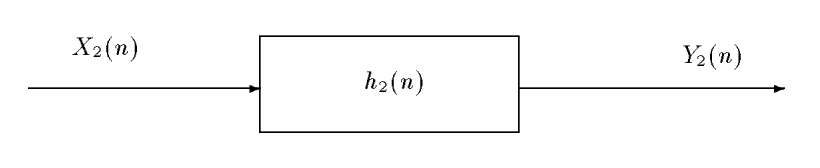
\includegraphics[width=10cm]{example.png}}
\caption{\label{fig:example} This is an example of figure included using LaTeX commands.}
\end{figure}
\end{listing}

which renders as

\begin{figure}[H]
\centerline{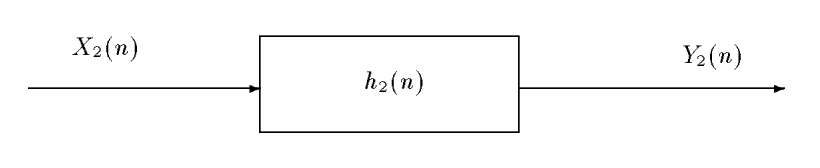
\includegraphics[width=10cm]{example.png}}
\caption{\label{fig:example} This is an example of figure included using LaTeX commands.}
\end{figure}

Of course, this Figure can now be referenced:

\begin{listing}
Figure \ref{fig:example} shows a second filter with input $X_2$, output $Y_2$  and an impulse response denoted as $h_2(n)$
\end{listing}

Figure \ref{fig:example} shows a second filter with input $X_2$,
output $Y_2$ and an impulse response denoted as $h_2(n)$

    \subsection{Other features}\label{other-features}

    \begin{itemize}
\itemsep1pt\parskip0pt\parsep0pt \item It is possible to mix LaTeX and
markdown markup in environments\textbackslash{} \item Environments can
be nested. However, this is not always perfect\ldots\{\}
\end{itemize}

    \subsection{User interface}\label{user-interface}

    \subsubsection{Buttons on main toolbar}\label{buttons-on-main-toolbar}

    On the main toolbar, the extension provides three buttons

\begin{figure}[H]
\centerline{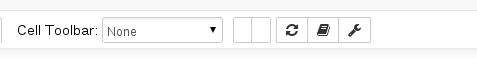
\includegraphics[width=10cm]{main_toolbar.png}}
\end{figure}

The first one can be used to refresh the numerotation of equations and
references in all the document. The second one fires the reading of the
bibliography bibtex file and creates (or updates) the reference section.
Finally the third one is a toogle button that opens or closes the
configuration toolbar.

    \subsubsection{Configuration toolbar}\label{configuration-toolbar}

    The configuration toolbar\\

\begin{figure}[H]
\centerline{
\includegraphics[width=10cm]{configuration_toolbar.png}}
\end{figure}

enables to enter some configuration options for the extension. First,
one can indicate the name of the bibtex file. If this file is not found
and the user creates the reference section, then this section will
indicate that the file was not found. The references drop-down menu
enables to choose the type of reference calls. The Equations input box
enable to initiate numbering of equations at the given number (this may
be useful for complex documents in several files/parts). Finally the
last drop-down menu let the user choose to number equation or to display
their label instead. These configuration options are then stored in the
notebook's metadata (and restored on reload).

    \section{Installation, usage and further
examples}\label{installation-usage-and-further-examples}

    \subsection{Installation}\label{installation}

    The extension consists in several javascript scripts:
\texttt{latex\_envs.js}, \texttt{thmsInNb4.js}, \texttt{bibInNb4.js} and
\texttt{initNb.js}, together with a stylesheet \texttt{latex\_envs.css}.
With Jupyter, you may also simply install the extension with

\begin{Shaded}
\begin{Highlighting}[]
\CharTok{from} \NormalTok{notebook.nbextensions }\CharTok{import} \NormalTok{install_nbextension, check_nbextension}
\NormalTok{install_nbextension(}\StringTok{"https://rawgit.com/jfbercher/latex_envs/master/latex_envs.zip"}\NormalTok{, user=}\OtherTok{True}\NormalTok{)}
\end{Highlighting}
\end{Shaded}

    An even more simple procedure is to issue

\begin{verbatim}
jupyter nbextension install https://rawgit.com/jfbercher/latex_envs/master/latex_envs.zip  --user
\end{verbatim}

at the command line.

    If you are still with IPython 3, you can install with

\begin{Shaded}
\begin{Highlighting}[]
\CharTok{from} \NormalTok{IPython.html.nbextensions }\CharTok{import} \NormalTok{install_nbextension, check_nbextension}
\NormalTok{install_nbextension(}\StringTok{"https://rawgit.com/jfbercher/latex_envs/master/latex_envs.zip"}\NormalTok{, user=}\OtherTok{True}\NormalTok{)}
\end{Highlighting}
\end{Shaded}

    You may then try the extension. Load it by typing

\begin{Shaded}
\begin{Highlighting}[]
\NormalTok{%%javascript}
\NormalTok{require(}\StringTok{"base/js/utils"}\NormalTok{).load_extensions(}\StringTok{"latex_envs/latex_envs"}\NormalTok{)}
\end{Highlighting}
\end{Shaded}

in a code cell of the notebook.

    If you want to automatically load the extension for any notebook, you
may use

\begin{Shaded}
\begin{Highlighting}[]
\CharTok{from} \NormalTok{IPython.html.services.config }\CharTok{import} \NormalTok{ConfigManager}
\NormalTok{ip = get_ipython()}
\NormalTok{cm = ConfigManager(parent=ip, profile_dir=ip.profile_dir.location)}
\NormalTok{cm.update(}\StringTok{'notebook'}\NormalTok{, \{}\StringTok{"load_extensions"}\NormalTok{: \{}\StringTok{"latex_envs/latex_envs"}\NormalTok{: }\OtherTok{True}\NormalTok{\}\})}
\end{Highlighting}
\end{Shaded}

    and replace the \texttt{True} by `None if you want to unload the
extension.

Alternatively you may also do this in javascript via

\begin{Shaded}
\begin{Highlighting}[]
\NormalTok{%%javascript}
\NormalTok{IPython.notebook.config.update(\{}\StringTok{"load_extensions"}\NormalTok{:\{}\StringTok{"latex_envs/latex_envs"}\NormalTok{:true\}\})}
\end{Highlighting}
\end{Shaded}

    replace the \texttt{true} by \texttt{null} to unload.

The last alternative is

\begin{verbatim}
jupyter nbextension enable latex_envs/latex_envs
\end{verbatim}

    and \texttt{disable} to disable it, of course.

    You may follow the instructions in the
\href{https://github.com/ipython-contrib/IPython-notebook-extensions/wiki}{wiki}
to install the extension.

    \subsection{First example (continued)}\label{first-example-continued}

    We continue the first example on fthe Fourier transform definition
\ref{def:FT} in order to show that, of course, we can illustrate things
using a simple code. Since the Fourier transform is an essential tool in
signal processing, We put this in evidence using the \texttt{textboxa}
environment -- which is defined here in the css, and that one should
define in the LaTeX counterpart:

\begin{listing}
\begin{textboxa}
The Fourier transform is an extremely useful tool to have in your toolbox!
\end{textboxa}
\end{listing}

    \begin{textboxa}
The Fourier transform is an extremely useful tool to have in your toolbox!
\end{textboxa}

    The Fourier transform of a pure cosine is given by \begin{equation}
X[k] = \frac{1}{2} \left( \delta[k-k_0] + \delta[k-k_0] \right), 
\end{equation} modulo $N$. This is illustrated in the following simple script:
% No prompt!
%\textbf{Input \#{}}%
\begin{lstlisting}
%matplotlib inline
import numpy as np
import matplotlib.pyplot as plt 
from numpy.fft import fft
k0=4; N=128; n=np.arange(N); k=np.arange(N)
x=np.sin(2*np.pi*k0*n/N)
X=fft(x)
plt.stem(k,np.abs(X))
plt.xlim([0, 20])
plt.title("Fourier transform of a cosine")
_=plt.xlabel("Frequency index (k)")
\end{lstlisting}% No prompt!
%\textbf{Output \#{}}
%
    \begin{center}
\adjustimage{max size={0.6\linewidth}{0.6\paperheight}}{latex_env_doc-ltx_tmp_files/latex_env_doc-ltx_tmp_46_0.png}
\end{center}
%    { \hspace*{\fill} \\}
    
    \subsection{Second example}\label{second-example}

    This example shows a series of environments, with different facets;
\textbf{links, references, markdown or/and LaTeX formatting within
environments}. Again, the rendering is done according to the stylesheet
\texttt{latex\_env.css}, which can be customized. The listing of
environments below is typed using the environment \emph{listing}\ldots{}

    \begin{listing}
\begin{definition} \label{def:diffeq}
We call \textbf{difference equation} an equation of the form
$$
\label{eq:diffeq}
y[n]= \sum_{k=1}^{p} a_k y[n-k] + \sum_{i=0}^q b_i x[n-i]
$$
\end{definition}

\begin{property}
If all the $a_k$ in equation (\ref{eq:diffeq}) of definition \ref{def:diffeq} are zero, then the filter has a **finite impulse response**. 
\end{property}

\begin{proof}
Let $\delta[n]$ denote the Dirac impulse. Take $x[n]=\delta[n]$ in (\ref{eq:diffeq}). This yields, by definition, the impulse response:
$$
\label{eq:fir}
h[n]= \sum_{i=0}^q b_i \delta[n-i],
$$
which has finite support. 
\end{proof}

\begin{theorem}
The poles of a causal stable filter are located within the unit circle in the complex plane.
\end{theorem}

\begin{example} \label{ex:IIR1}
Consider $y[n]= a y[n-1] +  x[n]$. The pole of the transfer function is $z=a$. The impulse response $h[n]=a^n$ has infinite support.
\end{example}

In the following exercise, you will check that the filter is stable iff $a$<1.

\begin{exercise}\label{ex:exofilter}
Consider the filter defined in Example \ref{ex:IIR1}. Using the **function** `lfilter` of scipy, compute and plot the impulse response for several values of $a$.
\end{exercise}

\end{listing}

    The lines above are rendered as follows (of course everything can be
tailored in the stylesheet):

\begin{definition}
\label{def:diffeq} We call \textbf{difference equation} an equation of
the form

\begin{equation}
\label{eq:diffeq}
y[n]= \sum_{k=1}^{p} a_k y[n-k] + \sum_{i=0}^q b_i x[n-i]
\end{equation}
\end{definition}

Properties of the filter are linked to the coefficients of the
difference equation. For instance, an immediate property is

\begin{property}
If all the $a_k$ in equation (\ref{eq:diffeq}) of definition
\ref{def:diffeq} are zero, then the filter has a \textbf{finite impulse
response}.
\end{property}

\begin{proof}
Let $\delta[n]$ denote the Dirac impulse. Take $x[n]=\delta[n]$ in
(\ref{eq:diffeq}). This yields, by definition, the impulse response:

\begin{equation}
\label{eq:fir}
h[n]= \sum_{i=0}^q b_i \delta[n-i],
\end{equation}

which has finite support.
\end{proof}

\begin{theorem}
The poles of a causal stable filter are located within the unit circle
in the complex plane.
\end{theorem}

\begin{example}
\label{ex:IIR1} Consider $y[n]= a y[n-1] + x[n]$. The pole of the
transfer function is $z=a$. The impulse response $h[n]=a^n$ has
infinite support.
\end{example}

In the following exercise, you will check that the filter is stable iff
$a$\textless{}1.

\begin{exercise}
\label{ex:exofilter} Consider the filter defined in Example
\ref{ex:IIR1}. Using the \textbf{function} \texttt{lfilter} of scipy,
compute and plot the impulse response for several values of $a$.
\end{exercise}

    \begin{listing}
The solution of exercise \ref{ex:exofilter}, which uses a difference equation as in Definition \ref{def:diffeq}:
\end{listing}

The solution of exercise \ref{ex:exofilter}, which uses a difference
equation as in Definition \ref{def:diffeq}:
% No prompt!
%\textbf{Input \#{}}%
\begin{lstlisting}
%matplotlib inline
import numpy as np
import matplotlib.pyplot as plt 
from scipy.signal import lfilter
d=np.zeros(100); d[0]=1 #dirac impulse
alist=[0.2, 0.8, 0.9, 0.95, 0.99, 0.999, 1.001, 1.01]
for a in alist:
    h=lfilter([1], [1, -a],d)
    _=plt.plot(h, label="a={}".format(a))
plt.ylim([0,1.5])
plt.xlabel('Time')
_=plt.legend()
\end{lstlisting}% No prompt!
%\textbf{Output \#{}}
%
    \begin{center}
\adjustimage{max size={0.6\linewidth}{0.6\paperheight}}{latex_env_doc-ltx_tmp_files/latex_env_doc-ltx_tmp_52_0.png}
\end{center}
%    { \hspace*{\fill} \\}
    
    \subsection{Third example:}\label{third-example}

    This example shows that environments like itemize or enumerate are also
available. As already indicated, this is useful for copying text from a
TeX file. Following the same idea, text formating commands
\texttt{\textbackslash{}textit}, \texttt{\textbackslash{}textbf},
\texttt{\textbackslash{}underline}, etc are also available.

    \begin{listing}
The following \textit{environments} are available:
\begin{itemize}
    \item \textbf{Theorems and likes}
    \begin{enumerate}
        \item theorem,
        \item lemma,
        \item corollary
        \item ...
    \end{enumerate}
    \item \textbf{exercises}
    \begin{enumerate}
        \item problem,
        \item example,
        \item exercise
    \end{enumerate}
\end{itemize}
\end{listing}

    which gives\ldots{}

The following \textit{environments} are available:

\begin{itemize}
\item \textbf{Theorems and likes}

\begin{enumerate}
\item theorem, \item lemma, \item corollary \item \ldots{}
\end{enumerate}

\item \textbf{exercises}

\begin{enumerate}
\item problem, \item example, \item exercise
\end{enumerate}
\end{itemize}

    \section{(post)-Converters}\label{post-converters}

    The extension works in the live-notebook. Since it relies on a bunch of
javascript, the notebook does not render as is in very nice services
such as \texttt{nbviewer} or \texttt{github} viewer. Similarly,
\texttt{nbconvert} does not know of the LaTeX constructs which are used
and therefore do not fully convert notebooks making use of this
extension. Therefore, it is necessary to add a post conversion step to
conversions provided by \texttt{nbconvert}. Though an interface exists
for adding post-converters to nbconvert, this (first) author was too
lazy and not enough strong to implement the post conversion along these
lines. What has be done are simple \texttt{bash} and \texttt{python}
scripts that perform this conversion.

    \subsection{Installation}\label{installation}

    Copy the scripts files to a directory in your search path, or launch the
scripts with the complete path. The two main scripts are
\texttt{ipynb\_thms\_to\_html} (conversion to html, of course:) and
\texttt{ipynb\_thms\_to\_latex} (conversion to LaTeX!).

    \subsection{Conversion to html}\label{conversion-to-html}

    \textbf{Requirements}: You will need \texttt{perl}, \texttt{nodejs}, and
\texttt{ipython3} (the script calls \texttt{ipython3}; if your
interpreter is \texttt{ipython}, edit the script and replace the
different occurences).

\textbf{Configuration}:

\begin{itemize}
\itemsep1pt\parskip0pt\parsep0pt \item If you still use IPython 3.x (not
Jupyter), edit \texttt{ipynb\_thms\_to\_html} and set the variable
\texttt{stillIPython3=true}. IPython 3.x will also have to change the
\texttt{nbextensionsDir} to \texttt{/.ipython/nbextensions} in the file
\texttt{post\_html\_thms.js}. \item Finally \textbf{all users} should
check the path for their \texttt{marked.js} library as indicated in
\texttt{post\_html\_thms.js}. On Debian, it is located
\texttt{/usr/share/jupyter/notebook/static/components/marked/lib/marked.js}.
It shoud be similar for other flavors of linux (may be
\texttt{/usr/local/share/...}). You may locate the right library by
issuing
\texttt{locate\ -eb0P\ marked.js\ \textbar{}\ xargs\ -r0\ ls\ -ald} on
the command line. Please update the variable \texttt{marked} for your
system in \texttt{post\_html\_thms.js}.
\end{itemize}

The conversion to html is done by something like

\begin{verbatim}
[path/]ipynb_thms_to_html filename
\end{verbatim}

or a list of files such as

\begin{verbatim}
[path/]ipynb_thms_to_html *.ipynb
\end{verbatim}

In turn, this script makes somes substitutions using \texttt{perl}, and
then uses the \texttt{nodesj} javascript interpreter to make the very
same substitutions that are done in the live notebook. The conversion
uses the template \texttt{thmsInNb.tpl} (located in the script
directory). It also copies the css \texttt{latex\_env.css} in the
directory of the output html file (it must be copied with html files in
the case of web upload).

    \subsection{Conversion to LaTeX}\label{conversion-to-latex}

    \textbf{Requirements}: You will need \texttt{perl} and
\texttt{ipython3}.

The conversion to LaTeX is done by something like

\begin{verbatim}
[path/]ipynb_thms_to_latex filename
\end{verbatim}

or a list of files such as

\begin{verbatim}
[path/]ipynb_thms_to_latex *.ipynb

\end{verbatim}

The script makes some substitutions and cleaning in markdown cells, then
calls the legacy \texttt{nbconvert}. Afterward, it runs through the
LaTeX environments and converts their contents (which can contain
markdown markup) to LaTeX. Note that the script contains a list of the
LaTeX environments to process. In the case of the addition of an
environment in the main javascript (\texttt{thmsInNb.js}), this list
must also be updated.

Finally, the script removes the header and footer in the LaTeX file.
This is a personnal choice, and the corresponding line can be safely
commented.

\begin{example}
As for an example, the present document has been converted using

\begin{verbatim}
ipynb_thms_to_latex latex_env_doc.ipynb
\end{verbatim}

Then the resulting file (without header/footer) has been included in the
main file \texttt{documentation.tex}, where some LaTeX definitions of
environments are done (namely listings, colors, etc) and compiled using

\begin{verbatim}
xelatex documentation
\end{verbatim}

The output can be consulted \href{documentation.pdf}{here}.
\end{example}

    \section{Disclaimer, sources and
thanks}\label{disclaimer-sources-and-thanks}

    This is a not-quick but certainly dirty hack. I am a complete beginner
in javascript and of course there are obviously a large amount of
possible improvements of the code, in cleaning, factorizing, etc!
Language also needs improvement.

\textbf{Contributions will be welcome and deeply appreciated.}

Originally, I used a piece of code from the nice online markdown editor
\texttt{stackedit}
\url{https://github.com/benweet/stackedit/issues/187}, where the authors
also considered the problem of incorporating LaTeX markup in their
markdown. I also used examples and code from
\url{https://github.com/ipython-contrib/IPython-notebook-extensions}.

    \section{References}\label{references}

(P'erez and Granger, 2007) P'erez Fernando and Granger Brian E.,
``\emph{IPython: a System for Interactive Scientific Computing}'',
Computing in Science and Engineering, vol.~9, number 3, pp.~21--29, May
2007. \href{http://ipython.org}{online}

(McKinney, 2012) Wes McKinney, ``\emph{Python for data analysis: Data
wrangling with Pandas, NumPy, and IPython}'', 2012.

(Rossant, 2013) Cyrille Rossant, ``\emph{Learning IPython for
interactive computing and data visualization}'', 2013.

(Shen, 2014) Shen Helen, ``\emph{Interactive notebooks: Sharing the
code}'', Nature, vol.~515, number 7525, pp.~151--152, 2014.


    % Add a bibliography block to the postdoc
    
    
%\bibliographystyle{ieetran}
%\bibliography{Thesis}

    
    